% ============================================================
%  DrowsyGuard - Edge-AI Driver Drowsiness Detection on Arduino UNO Q
%  Qualcomm Future Makers: Hack The Challenge 2026
%  Team ML_IoT_Love50 - HCMUT
%  Compile: xelatex main.tex  (run twice)
% ============================================================

\documentclass[aspectratio=169, 10pt]{beamer}
\usepackage{fontspec}
% ---- Typography ----
\setmainfont{Inter}
\setsansfont{Inter}
\setmonofont{DejaVu Sans Mono}[Scale=0.85]
\usepackage{beamerthemeMLIOT}

% ---- Additional packages ----
\usepackage{amsmath, amssymb}
\usepackage{booktabs}
\usepackage{colortbl}
\usepackage{caption}
\usepackage{hyperref}
\usepackage[loadonly]{enumitem}
\usepackage{array}
\usepackage{pifont}
\usepackage{ragged2e}
\usepackage{fontawesome5}
\usepackage{tikz}
\usepackage[skins]{tcolorbox}
\usetikzlibrary{arrows.meta, positioning, fit, backgrounds, shadows, calc}

\hypersetup{colorlinks=true, urlcolor=MLIOTaccent, linkcolor=MLIOTblue, citecolor=MLIOTblue}

% ---- Assets + competition (Qualcomm) palette ----
\graphicspath{{assets/}{./}}
\definecolor{QCblue}{HTML}{3253DC}   % Qualcomm blue
\definecolor{QCcyan}{HTML}{00A3E0}   % bright cyan accent
\definecolor{QCsky} {HTML}{E9F1FF}   % pale sky tint (background)
\definecolor{QCink} {HTML}{0A1B45}   % deep brand ink

% ---- Framed photo helper (white border + soft shadow) ----
\newcommand{\photo}[3][\linewidth]{%
  \begin{tikzpicture}
    \node[inner sep=0pt, line width=1.4pt, draw=white, rounded corners=2.5pt,
          drop shadow={shadow xshift=1.4pt, shadow yshift=-1.4pt, opacity=0.35, fill=black}]
      {\includegraphics[width=#1, height=#2, keepaspectratio]{#3}};
  \end{tikzpicture}}

% ============================================================
%  DESIGN SYSTEM (cards, chips, dividers) - shared with ML IoT deck
% ============================================================
\newtcolorbox{card}[2][]{enhanced, colback=MLIOTwhite, colframe=MLIOTnavy!22,
  boxrule=0.6pt, arc=2mm, boxsep=0.5mm, left=5pt, right=5pt, top=2.5pt, bottom=3pt,
  toptitle=2pt, bottomtitle=2pt,
  fonttitle=\footnotesize\bfseries, coltitle=MLIOTwhite, colbacktitle=MLIOTnavy,
  drop fuzzy shadow={black!35}, title={#2}, #1}

\newtcolorbox{goldcard}[2][]{enhanced, colback=MLIOTwhite, colframe=MLIOTgold!65,
  boxrule=0.6pt, arc=2mm, boxsep=0.5mm, left=5pt, right=5pt, top=2.5pt, bottom=3pt,
  toptitle=2pt, bottomtitle=2pt,
  fonttitle=\footnotesize\bfseries, coltitle=MLIOTnavy, colbacktitle=MLIOTgold,
  drop fuzzy shadow={black!35}, title={#2}, #1}

\newtcolorbox{alertcard}[2][]{enhanced, colback=MLIOTwhite, colframe=MLIOTcoral!55,
  boxrule=0.6pt, arc=2mm, boxsep=0.5mm, left=5pt, right=5pt, top=2.5pt, bottom=3pt,
  toptitle=2pt, bottomtitle=2pt,
  fonttitle=\footnotesize\bfseries, coltitle=MLIOTwhite, colbacktitle=MLIOTcoral,
  drop fuzzy shadow={black!35}, title={#2}, #1}

% ---- Chips ----
\newcommand{\chip}[2]{\tikz[baseline=(t.base)]{\node[rounded corners=2.6pt, fill=#1,
  text=MLIOTwhite, font=\tiny\bfseries, inner xsep=5.5pt, inner ysep=2.4pt] (t) {#2};}}
\newcommand{\chipgold}[1]{\tikz[baseline=(t.base)]{\node[rounded corners=2.6pt, fill=MLIOTgold,
  text=MLIOTnavy, font=\tiny\bfseries, inner xsep=5.5pt, inner ysep=2.4pt] (t) {#1};}}

% ---- Section divider (English, Qualcomm co-brand) ----
\newcommand{\sectiondivider}[2]{%
\begin{frame}[plain]
  \begin{tikzpicture}[remember picture, overlay]
    \shade[top color=QCink, bottom color=MLIOTnavy]
      (current page.north west) rectangle (current page.south east);
    % decorative diagonal accents
    \fill[QCcyan, opacity=0.13] (current page.north east) -- ++(-4.2,0) -- ++(4.2,-4.2) -- cycle;
    \fill[MLIOTgold, opacity=0.10] (current page.south west) -- ++(3.6,0) -- ++(-3.6,3.6) -- cycle;
    % ghost number
    \node[text=white, opacity=0.08, font=\fontsize{195}{195}\selectfont\bfseries, anchor=south east]
      at ([xshift=-0.2cm, yshift=0.2cm]current page.south east) {#1};
    % top co-brand: ML IoT left, Qualcomm right
    \node[anchor=west] at ([xshift=0.7cm, yshift=-0.7cm]current page.north west)
      {
\includegraphics[height=0.62cm]{mliot_banner.png}};
    \node[anchor=east] at ([xshift=-0.7cm, yshift=-0.7cm]current page.north east)
      {
\includegraphics[height=0.6cm]{qualcomm_white.png}};
    % PART chip
    \node[fill=MLIOTgold, text=QCink, font=\normalsize\bfseries, rounded corners=3pt,
          inner xsep=11pt, inner ysep=4.5pt, anchor=west]
      at ([xshift=1.3cm, yshift=1.0cm]current page.west) {PART #1};
    % title
    \node[text=white, font=\LARGE\bfseries, anchor=west, text width=11.5cm, align=left]
      at ([xshift=1.3cm, yshift=-0.3cm]current page.west) {#2};
    % accent gradient line
    \shade[left color=QCcyan, right color=MLIOTgold]
      ([xshift=1.3cm, yshift=-1.15cm]current page.west) rectangle
      ([xshift=6.0cm, yshift=-1.22cm]current page.west);
  \end{tikzpicture}
\end{frame}}

% ---- Reusable TikZ styles ----
\tikzset{
  box/.style={draw=MLIOTnavy, line width=1.1pt, fill=MLIOTbglight, rounded corners=3pt,
              minimum height=1.15cm, text width=2.5cm, align=center, font=\footnotesize\bfseries,
              drop shadow={shadow xshift=1.1pt, shadow yshift=-1.1pt, opacity=0.22, fill=black}},
  boxhi/.style={draw=MLIOTcoral, line width=1.4pt, fill=MLIOTlight, rounded corners=3pt,
              minimum height=1.15cm, text width=2.5cm, align=center, font=\footnotesize\bfseries,
              drop shadow={shadow xshift=1.1pt, shadow yshift=-1.1pt, opacity=0.22, fill=black}},
  lbl/.style={font=\scriptsize\bfseries, MLIOTnavy},
  arr/.style={-{Latex[length=2.6mm, width=1.9mm]}, line width=1.1pt, MLIOTnavy},
}

\newcommand{\thead}[1]{\textcolor{MLIOTwhite}{\textbf{\footnotesize #1}}}

% ============================================================
%  REDESIGN: background, branded header ribbon, footer
% ============================================================
% ---- Soft sky-tint gradient background (all content slides) ----
\setbeamertemplate{background}{%
  \begin{tikzpicture}[remember picture, overlay]
    \shade[top color=white, bottom color=QCsky] (current page.north west) rectangle (current page.south east);
    % faint decorative corner accent (bottom-right, behind content)
    \fill[QCcyan, opacity=0.06] (current page.south east) -- ++(-3.0,0) -- ++(3.0,3.0) -- cycle;
  \end{tikzpicture}%
}

% ---- Frame title: co-brand ribbon + title below ----
\setbeamertemplate{frametitle}{%
  \begin{tikzpicture}[remember picture, overlay]
    % navy ribbon
    \fill[MLIOTnavy] (current page.north west) rectangle ([yshift=-0.9cm] current page.north east);
    % gradient accent line (cyan -> gold)
    \shade[left color=QCcyan, right color=MLIOTgold]
      ([yshift=-0.9cm] current page.north west) rectangle ([yshift=-0.95cm] current page.north east);
    % ML IoT wordmark (left)
    \node[anchor=west] at ([xshift=0.42cm, yshift=-0.45cm] current page.north west)
      {
\includegraphics[height=0.52cm]{mliot_banner.png}};
    % Qualcomm logo (right, dominant sponsor)
    \node[anchor=east] at ([xshift=-0.42cm, yshift=-0.45cm] current page.north east)
      {
\includegraphics[height=0.52cm]{qualcomm_white.png}};
    % gold accent tab + frame title below the ribbon
    \fill[MLIOTgold, rounded corners=1pt]
      ([xshift=0.5cm, yshift=-1.22cm] current page.north west) rectangle
      ([xshift=0.64cm, yshift=-1.62cm] current page.north west);
    \node[anchor=west, text=MLIOTnavy, font=\Large\bfseries, text width=13cm, align=left]
      at ([xshift=0.82cm, yshift=-1.43cm] current page.north west) {\insertframetitle};
  \end{tikzpicture}%
  \vspace{1.34cm}
}

% ---- Footer: branded, with competition hashtag ----
\setbeamertemplate{footline}{%
  \begin{beamercolorbox}[wd=\paperwidth, ht=0.5cm, dp=0.18cm,
        leftskip=0.42cm, rightskip=0.42cm]{footline}%
    \usebeamerfont{footline}%
    \rlap{\textbf{DrowsyGuard}}%
    \hfill \textcolor{MLIOTgold}{\#}QualcommHackTheChallenge2026 \hfill
    \llap{\insertframenumber}%
  \end{beamercolorbox}%
}

% ============================================================
%  METADATA
% ============================================================
\title{DrowsyGuard\\[0.2em]
\large Edge-AI Driver Drowsiness Detection on Arduino UNO Q}

\author{%
  \textbf{\textcolor{MLIOTnavy}{Nguyen Hoang Trieu} $\cdot$
  \textcolor{MLIOTnavy}{Tang Phon Thinh} $\cdot$
  \textcolor{MLIOTnavy}{Van Dac Phong Truc} $\cdot$
  \textcolor{MLIOTnavy}{Vo Phuc Thinh}}%
}

\setAffiliations{%
  Platform: \textbf{Arduino UNO Q} -- Qualcomm Dragonwing QRB2210 (Linux) + STM32U585 (MCU)%
}

\institute{%
  Team ML\_IoT\_Love50 -- Qualcomm Future Makers: Hack The Challenge 2026%
}

\date{}

% ============================================================
\begin{document}

% ============================================================
%  BODY - organised around the 4 judging criteria
%   1. Problem statement        (Mo ta van de can giai quyet)
%   2. Product description      (Mo ta san pham)
%   3. Technical readiness      (Muc do ky thuat san sang)
%   4. Application domains      (Linh vuc ap dung)
% ============================================================

% ------------------------------------------------------------
%  TITLE
% ------------------------------------------------------------
\begin{frame}[plain]
  \begin{tikzpicture}[remember picture, overlay]
    \shade[top color=QCink, bottom color=MLIOTnavy]
      (current page.north west) rectangle (current page.south east);
    \node[anchor=west] at ([xshift=0.7cm, yshift=-0.85cm]current page.north west)
      {
\includegraphics[height=0.92cm]{mliot_banner.png}};
    \node[anchor=east] at ([xshift=-0.7cm, yshift=-0.85cm]current page.north east)
      {
\includegraphics[height=0.92cm]{qualcomm_white.png}};
    \shade[left color=QCcyan, right color=MLIOTgold]
      ([yshift=-1.55cm]current page.north west) rectangle ([yshift=-1.60cm]current page.north east);
    \begin{scope}
      \clip ([yshift=-1.60cm]current page.north west) rectangle ([yshift=-4.80cm]current page.north east);
      \node[anchor=north] at ([yshift=-1.60cm]current page.north)
        {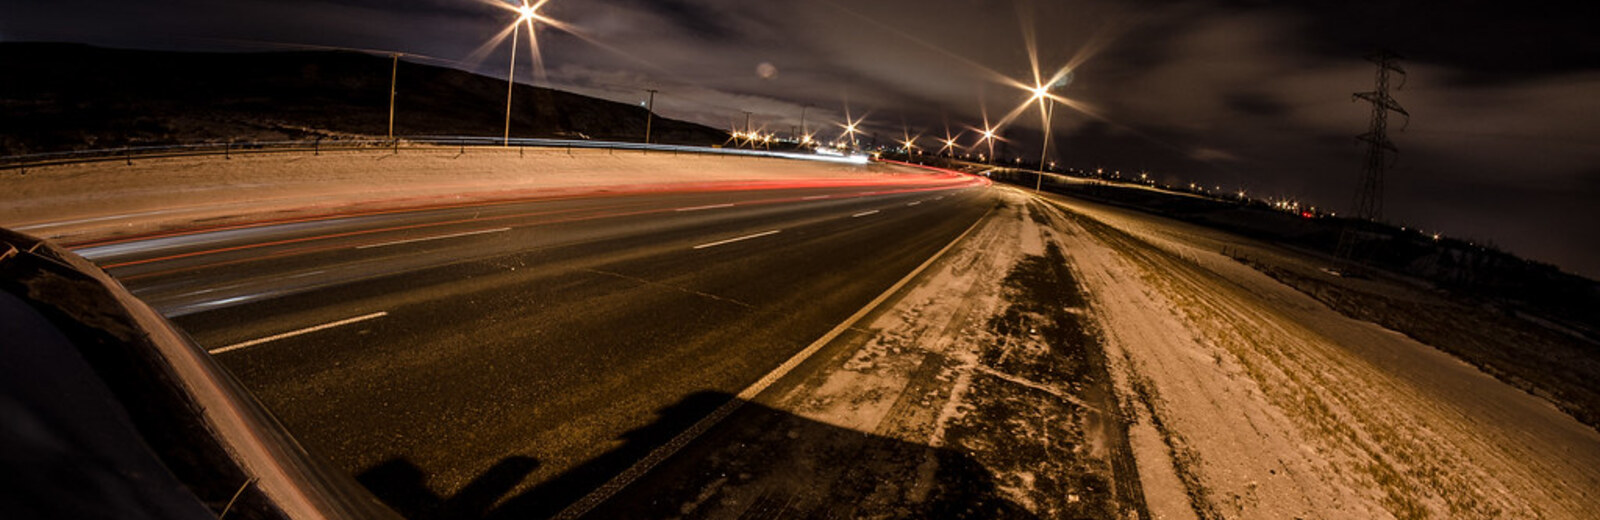
\includegraphics[width=\paperwidth, height=3.3cm]{hero_night.jpg}};
      \fill[QCink, opacity=0.34]
        ([yshift=-1.60cm]current page.north west) rectangle ([yshift=-4.80cm]current page.north east);
    \end{scope}
    \fill[MLIOTgold] ([yshift=-4.80cm]current page.north west) rectangle ([yshift=-4.85cm]current page.north east);
    \node[anchor=north, text=white, font=\fontsize{32}{34}\selectfont\bfseries]
      at ([yshift=-5.20cm]current page.north) {Drowsy\textcolor{QCcyan}{Guard}};
    \node[anchor=north, text=MLIOTgold, font=\normalsize\bfseries, text width=13cm, align=center]
      at ([yshift=-6.55cm]current page.north) {Edge-AI Driver Drowsiness Detection on Arduino UNO Q};
    \node[anchor=north, text=white, align=center, text width=13.8cm]
      at ([yshift=-7.18cm]current page.north)
      {\footnotesize\mbox{\textbf{Nguyen Hoang Trieu}}~~\textcolor{QCcyan}{$\bullet$}~~\mbox{\textbf{Tang Phon Thinh}}~~\textcolor{QCcyan}{$\bullet$}~~\mbox{\textbf{Van Dac Phong Truc}}~~\textcolor{QCcyan}{$\bullet$}~~\mbox{\textbf{Vo Phuc Thinh}}};
    \draw[MLIOTgold, line width=0.6pt]
      ([xshift=-2.7cm, yshift=-7.66cm]current page.north) -- ([xshift=2.7cm, yshift=-7.66cm]current page.north);
    \node[anchor=north, text=QCsky, font=\scriptsize, align=center, text width=13.8cm]
      at ([yshift=-7.80cm]current page.north)
      {Platform: \textbf{\textcolor{white}{Arduino UNO Q}} -- Qualcomm Dragonwing QRB2210 (Linux) + STM32U585 (MCU)};
    \node[anchor=south, fill=MLIOTgold, text=QCink, rounded corners=3pt, inner xsep=10pt, inner ysep=4pt,
          font=\scriptsize\bfseries] at ([yshift=0.28cm]current page.south)
      {Qualcomm Future Makers: Hack The Challenge 2026 ~~$\cdot$~~ Team ML\_IoT\_Love50};
  \end{tikzpicture}
\end{frame}

% ------------------------------------------------------------
%  AGENDA = the four judging criteria
% ------------------------------------------------------------
\begin{frame}{Agenda}
  \vspace{0.3em}
  \begin{columns}[T]
    \begin{column}{0.24\textwidth}
      \begin{card}{\faExclamationTriangle~~PART 1}
        \scriptsize \textbf{The Problem}\\[2pt] What we are solving and who suffers from it.
      \end{card}
    \end{column}
    \begin{column}{0.24\textwidth}
      \begin{card}{\faBoxOpen~~PART 2}
        \scriptsize \textbf{The Product}\\[2pt] What DrowsyGuard is, does and how it is built.
      \end{card}
    \end{column}
    \begin{column}{0.24\textwidth}
      \begin{card}{\faCheckCircle~~PART 3}
        \scriptsize \textbf{Technical Readiness}\\[2pt] What already works and what is left.
      \end{card}
    \end{column}
    \begin{column}{0.24\textwidth}
      \begin{card}{\faGlobeAsia~~PART 4}
        \scriptsize \textbf{Application Domains}\\[2pt] Where it applies and how far it scales.
      \end{card}
    \end{column}
  \end{columns}

  \vspace{1.1em}
  \begin{center}
  \begin{tikzpicture}
    \node[box, fill=MLIOTnavy, text=MLIOTwhite, draw=MLIOTnavy, text width=3.0cm] (a) {\faVideo\\[2pt]Camera sees\\ the driver};
    \node[box, right=0.7cm of a, text width=3.0cm] (b) {\faBrain\\[2pt]Edge AI detects\\ drowsiness};
    \node[boxhi, right=0.7cm of b, text width=3.0cm] (c) {\faBell\\[2pt]Escalating\\ alert \& control};
    \draw[arr] (a) -- (b);
    \draw[arr, MLIOTcoral] (b) -- (c);
  \end{tikzpicture}
  \end{center}
  \vspace{0.5em}
  \centering
  \chipgold{100\% on-device}\hspace{0.4em}\chipgold{No internet needed}\hspace{0.4em}\chipgold{Privacy preserved}
\end{frame}

% ============================================================
\sectiondivider{1}{The Problem We Solve}
% ============================================================

% ------------------------------------------------------------
\begin{frame}{Drowsy driving is a silent killer}
  \begin{columns}[T]
    \begin{column}{0.54\textwidth}
      \begin{card}{\faExclamationTriangle~~Why it matters}
        \scriptsize
        \begin{itemize}
          \item Fatigue and micro-sleep are among the leading causes of severe road accidents worldwide.
          \item Highest risk for \textbf{long-haul truck, coach and ride-hailing drivers}, especially at night.
          \item A micro-sleep of just \textbf{3--4 seconds} at 90\,km/h means driving \textbf{blind for 100\,m}.
        \end{itemize}
      \end{card}
      \vspace{0.4em}
      \begin{alertcard}{\faRoad~~Vietnam context}
        \scriptsize Insert local statistics on fatigue-related traffic accidents here (source to be cited). The pain is concrete and nationwide.
      \end{alertcard}
    \end{column}
    \begin{column}{0.44\textwidth}
      \centering
      \photo[\linewidth]{4.5cm}{problem_driver.jpg}\\[0.3em]
      {\scriptsize\itshape A fatigued driver at the wheel, late at night.}
    \end{column}
  \end{columns}
\end{frame}

% ------------------------------------------------------------
\begin{frame}{Who suffers from it}
  \vspace{0.3em}
  \begin{columns}[T]
    \begin{column}{0.32\textwidth}
      \begin{card}{\faTruck~~Long-haul drivers}
        \scriptsize Night runs, tight delivery windows, hours alone at the wheel. The highest-risk group.
      \end{card}
    \end{column}
    \begin{column}{0.32\textwidth}
      \begin{card}{\faBus~~Coach \& bus operators}
        \scriptsize Dozens of passengers per vehicle -- one micro-sleep becomes a mass-casualty event.
      \end{card}
    \end{column}
    \begin{column}{0.32\textwidth}
      \begin{card}{\faCarSide~~Ride-hailing \& private}
        \scriptsize Long shifts to hit income targets, often after a full working day.
      \end{card}
    \end{column}
  \end{columns}
  \vspace{1.0em}
  \begin{center}
    \begin{goldcard}[width=0.92\textwidth]{\faBuilding~~And the businesses behind them}
      \small Fleet and logistics operators carry the cost: vehicle damage, cargo loss, insurance premiums, driver injury and reputational damage after every fatigue incident.
    \end{goldcard}
  \end{center}
\end{frame}

% ------------------------------------------------------------
\begin{frame}{Existing solutions leave a gap}
  \vspace{0.2em}
  \centering
  \renewcommand{\arraystretch}{1.45}
  \small
  \begin{tabular}{@{}p{4.0cm}p{4.0cm}p{4.4cm}@{}}
    \rowcolor{MLIOTnavy}\thead{Approach} & \thead{Limitation} & \thead{Consequence} \\
    Built-in driver monitoring on premium cars & Only on expensive vehicles & Out of reach for most drivers \\
    \rowcolor{MLIOTbglight} Cloud dashcam analytics & Needs network, adds latency & Fails on rural roads, feels intrusive \\
    Wearables (smart bands, caps) & Uncomfortable, easy to forget & Low adoption in practice \\
  \end{tabular}

  \vspace{1.0em}
  \begin{columns}
    \begin{column}{0.9\textwidth}
      \begin{goldcard}{\faBullseye~~The unmet need}
        \small A \textbf{low-cost add-on device} that runs \textbf{fully on-device}, works \textbf{offline}, protects \textbf{privacy}, and fits \textbf{any vehicle}.
      \end{goldcard}
    \end{column}
  \end{columns}
\end{frame}

% ============================================================
\sectiondivider{2}{The Product}
% ============================================================

% ------------------------------------------------------------
\begin{frame}{DrowsyGuard in one line}
  \vspace{0.3em}
  \begin{center}
    \begin{goldcard}[width=0.9\textwidth]{\faLightbulb~~Concept}
      \normalsize A small dashboard device that \textbf{watches the driver with a camera}, detects drowsiness \textbf{on the edge}, and triggers an \textbf{escalating alert} before it is too late.
    \end{goldcard}
  \end{center}
  \vspace{0.6em}
  \begin{columns}[T]
    \begin{column}{0.32\textwidth}
      \begin{card}{\faBrain~~Perceive}
        \scriptsize Retrained YOLO detects eyes, yawns and head nods in real time on the Linux core.
      \end{card}
    \end{column}
    \begin{column}{0.32\textwidth}
      \begin{card}{\faChartLine~~Decide}
        \scriptsize PERCLOS, yawn rate and nod count are fused into a drowsiness level 0--3.
      \end{card}
    \end{column}
    \begin{column}{0.32\textwidth}
      \begin{card}{\faBell~~Act}
        \scriptsize The MCU escalates the alert: beep, then haptics, then full alarm and SOS.
      \end{card}
    \end{column}
  \end{columns}
  \vspace{0.5em}
  \centering
  \chip{MLIOTnavy}{Low latency}\hspace{0.4em}\chip{MLIOTnavy}{Offline}\hspace{0.4em}\chip{MLIOTcoral}{Private by design}\hspace{0.4em}\chipgold{Fits any car}
\end{frame}

% ------------------------------------------------------------
\begin{frame}{What the product looks like}
  \begin{columns}[T]
    \begin{column}{0.5\textwidth}
      \centering
      \begin{tikzpicture}[scale=1.0, font=\scriptsize]
        \fill[QCcyan!12, rounded corners=10pt] (-1.95,-0.55) rectangle (1.95,2.25);
        \fill[MLIOTnavy, rounded corners=7pt] (-1.6,-0.2) rectangle (1.6,2.05);
        \fill[MLIOTlight] (0,1.75) circle (0.17);
        \fill[QCblue] (0,1.75) circle (0.09);
        \fill[white] (0.05,1.80) circle (0.028);
        \fill[green!60!black] (-1.18,1.75) circle (0.085);
        \fill[MLIOTgold]      (-0.82,1.75) circle (0.085);
        \fill[MLIOTcoral]     ( 1.18,1.75) circle (0.085);
        \fill[QCink, rounded corners=4pt] (-1.36,0.08) rectangle (1.36,1.4);
        \fill[QCcyan] (-0.43,0.92) circle (0.1);
        \fill[QCcyan] ( 0.43,0.92) circle (0.1);
        \draw[QCcyan, line width=1.3pt] (-0.33,0.52) .. controls (0,0.34) .. (0.33,0.52);
        \node[text=white, font=\tiny\bfseries] at (0,0.24) {DRIVER OK};
      \end{tikzpicture}\\[0.3em]
      \photo[\linewidth]{2.1cm}{car_dashboard.jpg}\\[0.12em]
      {\scriptsize Compact unit mounts on the dashboard, camera facing the driver.}
    \end{column}
    \begin{column}{0.48\textwidth}
      \begin{card}{\faSlidersH~~Simple status interface}
        \scriptsize
        \begin{itemize}
          \item \textcolor{green!55!black}{\faCircle}~Green: driver alert.
          \item \textcolor{MLIOTgold}{\faCircle}~Amber: early drowsiness.
          \item \textcolor{MLIOTcoral}{\faCircle}~Red: danger, full alarm.
        \end{itemize}
      \end{card}
      \vspace{0.4em}
      \begin{goldcard}{\faPlug~~Zero-friction UX}
        \scriptsize Plug into 12\,V power and it just runs. No pairing, no app setup, no driver action required.
      \end{goldcard}
    \end{column}
  \end{columns}
\end{frame}

% ------------------------------------------------------------
\begin{frame}{How it works: end to end}
  \vspace{0.4em}
  \begin{center}
  \begin{tikzpicture}[font=\footnotesize]
    \def\dx{3.55}
    \foreach \i in {0,1,2}{
      \pgfmathsetmacro{\xa}{\i*\dx+0.72}
      \pgfmathsetmacro{\xb}{(\i+1)*\dx-0.72}
      \ifnum\i=2
        \draw[-{Latex[length=2.6mm,width=2mm]}, line width=1.6pt, MLIOTcoral!85] (\xa,0) -- (\xb,0);
      \else
        \draw[-{Latex[length=2.6mm,width=2mm]}, line width=1.6pt, MLIOTnavy!35] (\xa,0) -- (\xb,0);
      \fi
    }
    \foreach \i/\col/\ic/\ti/\su in {%
        0/MLIOTnavy/{\faVideo}/Capture/{driver face},
        1/QCblue/{\faBrain}/Analyze/{YOLO on Linux},
        2/QCcyan/{\faChartLine}/Score/{level 0--3},
        3/MLIOTcoral/{\faBell}/Act/{alert + control}}{
      \pgfmathsetmacro{\x}{\i*\dx}
      \pgfmathtruncatemacro{\n}{\i+1}
      \fill[\col, opacity=0.14] (\x,0) circle (0.8);
      \shade[inner color=\col!85, outer color=\col] (\x,0) circle (0.62);
      \node[text=white, font=\Large] at (\x,0) {\ic};
      \node[circle, fill=white, draw=\col, line width=0.8pt, text=\col, font=\tiny\bfseries,
            inner sep=0.4pt, minimum size=0.42cm] at (\x+0.5,0.5) {\n};
      \node[text=MLIOTnavy, font=\footnotesize\bfseries] at (\x,-1.08) {\ti};
      \node[text=MLIOTink!75, font=\tiny] at (\x,-1.4) {\su};
    }
  \end{tikzpicture}
  \end{center}
  \vspace{0.6em}
  \begin{columns}[T]
    \begin{column}{0.48\textwidth}
      \begin{card}{\faLock~~Everything stays on the device}
        \scriptsize No frame ever leaves the unit. All four steps run locally, so the system reacts instantly and keeps the driver's face private.
      \end{card}
    \end{column}
    \begin{column}{0.48\textwidth}
      \begin{goldcard}{\faBolt~~Reaction budget}
        \scriptsize Target end-to-end latency \textbf{under 200\,ms} from eyes closing to the first alert -- impossible to guarantee over the cloud.
      \end{goldcard}
    \end{column}
  \end{columns}
\end{frame}

% ------------------------------------------------------------
\begin{frame}{System architecture: the dual-brain board}
  \vspace{0.3em}
  \begin{center}
  \begin{tikzpicture}[font=\scriptsize]
    \def\py{1.55}\def\pY{-1.55}
    \shade[inner color=MLIOTnavy, outer color=QCink] (-0.92,-0.72) rectangle (0.92,0.72);
    \draw[MLIOTnavy, line width=1pt, rounded corners=6pt] (-0.92,-0.72) rectangle (0.92,0.72);
    \node[text=white, font=\large] at (0,0.3) {\faVideo};
    \node[text=white, font=\footnotesize\bfseries] at (0,-0.14) {Camera};
    \node[text=QCcyan!85, font=\scriptsize] at (0,-0.48) {RGB / IR};

    \def\lx{2.25}\def\lX{6.5}
    \fill[white, rounded corners=6pt] (\lx,\pY) rectangle (\lX,\py);
    \fill[MLIOTnavy, rounded corners=6pt] (\lx,\py-0.68) rectangle (\lX,\py);
    \fill[MLIOTnavy] (\lx,\py-0.68) rectangle (\lX,\py-0.38);
    \draw[MLIOTnavy, line width=1.3pt, rounded corners=6pt] (\lx,\pY) rectangle (\lX,\py);
    \node[text=white, font=\footnotesize\bfseries] at ({(\lx+\lX)/2},\py-0.34) {\faBrain~~Linux $\cdot$ QRB2210};
    \node[anchor=north west, text=MLIOTink, align=left, font=\scriptsize, text width=3.85cm] at (\lx+0.2,\py-0.86)
      {\textbf{YOLO} eye \& face detect\\[3pt] PERCLOS $\cdot$ yawn $\cdot$ nod\\[3pt] Drowsiness level 0--3\\[3pt] GPS $\cdot$ SMS $\cdot$ dashboard};

    \def\mx{7.6}\def\mX{11.4}
    \fill[white, rounded corners=6pt] (\mx,\pY) rectangle (\mX,\py);
    \fill[MLIOTcoral, rounded corners=6pt] (\mx,\py-0.68) rectangle (\mX,\py);
    \fill[MLIOTcoral] (\mx,\py-0.68) rectangle (\mX,\py-0.38);
    \draw[MLIOTcoral, line width=1.3pt, rounded corners=6pt] (\mx,\pY) rectangle (\mX,\py);
    \node[text=white, font=\footnotesize\bfseries] at ({(\mx+\mX)/2},\py-0.34) {\faMicrochip~~MCU $\cdot$ STM32U585};
    \node[anchor=north west, text=MLIOTink, align=left, font=\scriptsize, text width=3.45cm] at (\mx+0.2,\py-0.86)
      {\textbf{Real-time} $<$100\,ms\\[3pt] Buzzer $\cdot$ vibration\\[3pt] Fan relay $\cdot$ status LED\\[3pt] ``I am awake'' button};

    \def\ay{-2.95}
    \fill[MLIOTbglight, rounded corners=5pt] (\mx,\ay-0.52) rectangle (\mX,\ay+0.5);
    \draw[MLIOTnavy!30, line width=1pt, rounded corners=5pt] (\mx,\ay-0.52) rectangle (\mX,\ay+0.5);
    \node[text=MLIOTnavy, font=\scriptsize\bfseries] at ({(\mx+\mX)/2},\ay+0.3) {Actuators};
    \foreach \k/\ic in {0/{\faVolumeUp},1/{\faBell},2/{\faSnowflake},3/{\faLightbulb}}{
      \pgfmathsetmacro{\cx}{\mx+0.86+\k*0.74}
      \node[circle, fill=white, draw=MLIOTcoral!60, line width=0.7pt, text=MLIOTcoral,
            minimum size=0.54cm, inner sep=0pt, font=\scriptsize] at (\cx,\ay-0.14) {\ic};
    }

    \draw[arr, line width=1.5pt] (0.92,0) -- (\lx,0);
    \draw[arr, line width=1.5pt] (\lX,0) -- (\mx,0);
    \node[fill=MLIOTgold, text=QCink, rounded corners=2pt, inner xsep=3pt, inner ysep=1pt, font=\tiny\bfseries]
      at ({(\lX+\mx)/2},0.18) {Bridge};
    \node[text=MLIOTnavy!85, font=\tiny] at ({(\lX+\mx)/2},-0.26) {level 0--3};
    \draw[arr, MLIOTcoral, line width=1.5pt] ({(\mx+\mX)/2},\pY) -- ({(\mx+\mX)/2},\ay+0.5);
  \end{tikzpicture}
  \end{center}
  \vspace{0.3em}
  \centering
  \chipgold{\faLightbulb~~Linux for heavy AI, MCU for instant control -- one Arduino UNO Q board does both}
\end{frame}

% ------------------------------------------------------------
\begin{frame}{Escalating alert ladder}
  \vspace{-0.1em}
  \begin{center}
  \begin{tikzpicture}[font=\scriptsize\bfseries]
    \def\w{3.0}\def\h{0.78}\def\stp{2.55}
    \foreach \i/\c/\t/\d in {%
      0/MLIOTnavy!55/{L0 Normal}/{Silent, green LED},
      1/MLIOTgold/{L1 Early}/{Beep, amber LED},
      2/MLIOTcoral/{L2 Drowsy}/{Alarm, haptics, fan},
      3/MLIOTcoral!70!black/{L3 Danger}/{Hazard, slowdown, SOS}}{
      \pgfmathsetmacro{\x}{\i*\stp}
      \pgfmathsetmacro{\y}{\i*(\h+0.05)}
      \fill[\c, rounded corners=3pt, drop shadow={opacity=0.25}] (\x,\y) rectangle ++(\w,\h);
      \node[text=white, align=center, text width=2.7cm] at (\x+\w/2,\y+\h/2) {\t\\[0.5pt]\tiny\mdseries\d};
    }
    \draw[arr, MLIOTcoral, line width=1.3pt] (0.35,-0.35) -- node[below=1pt, lbl, font=\tiny\bfseries, pos=0.5]{increasing drowsiness} (10.3,-0.35);
  \end{tikzpicture}
  \end{center}
  \vspace{0.1em}
  \centering
  \begin{goldcard}[width=0.9\textwidth]{\faBell~~Design principle}
    \scriptsize Gentle enough not to startle, strong enough to wake. The driver presses \textbf{``I am awake''} to reset.
  \end{goldcard}
\end{frame}

% ------------------------------------------------------------
\begin{frame}{Control functions}
  \begin{columns}[T]
    \begin{column}{0.5\textwidth}
      \begin{card}{\faMicrochip~~On the MCU -- real time}
        \scriptsize
        \begin{itemize}
          \item Buzzer and voice warning.
          \item Vibration motor in seat / steering.
          \item Relay for cool-air fan.
          \item Three-color status LED.
          \item ``I am awake'' acknowledge button.
          \item GPIO/CAN signal to cut throttle or flash hazards.
        \end{itemize}
      \end{card}
    \end{column}
    \begin{column}{0.5\textwidth}
      \begin{goldcard}{\faSatelliteDish~~On Linux -- connectivity}
        \scriptsize
        \begin{itemize}
          \item Log drowsiness events with time + GPS.
          \item Send SOS via SMS / 4G if unresponsive.
          \item Fleet dashboard with per-driver safety score.
          \item Per-driver threshold personalization.
        \end{itemize}
      \end{goldcard}
      \vspace{0.4em}
      \begin{alertcard}{\faUsers~~Fleet value}
        \scriptsize Logistics companies get a safety tool, not just a gadget.
      \end{alertcard}
    \end{column}
  \end{columns}
\end{frame}

% ------------------------------------------------------------
\begin{frame}{Hardware and cost}
  \begin{columns}[T]
    \begin{column}{0.56\textwidth}
      \centering
      \renewcommand{\arraystretch}{1.35}
      \scriptsize
      \begin{tabular}{@{}p{4.3cm}p{2.6cm}@{}}
        \rowcolor{MLIOTnavy}\thead{Component} & \thead{Role} \\
        Arduino UNO Q & Compute (AI + MCU) \\
        \rowcolor{MLIOTbglight} RGB + IR camera & Day/night capture \\
        Buzzer + speaker & Audio alert \\
        \rowcolor{MLIOTbglight} Vibration motor & Haptic alert \\
        Fan + relay & Cool-air wake-up \\
        \rowcolor{MLIOTbglight} GPS + status LED & Location + UI \\
      \end{tabular}
    \end{column}
    \begin{column}{0.42\textwidth}
      \centering
      \photo[\linewidth]{3.0cm}{arduino_unoq.png}\\[0.3em]
      \begin{goldcard}{\faDollarSign~~Cost position}
        \scriptsize A \textbf{low-cost add-on}, a fraction of the price of built-in premium driver-monitoring systems. One self-contained unit, powered from the 12\,V socket.
      \end{goldcard}
    \end{column}
  \end{columns}
\end{frame}

% ============================================================
\sectiondivider{3}{Technical Readiness}
% ============================================================

% ------------------------------------------------------------
%  TRL SCALE  (Muc do ky thuat san sang)
% ------------------------------------------------------------
\begin{frame}{Where we stand: Technology Readiness Level}
  \vspace{0.6em}
  \begin{center}
  \begin{tikzpicture}[font=\tiny]
    \def\bw{1.18}
    \foreach \i in {1,...,9}{
      \pgfmathsetmacro{\x}{(\i-1)*\bw}
      \pgfmathsetmacro{\hh}{0.30+\i*0.105}
      \pgfmathsetmacro{\bwi}{\bw-0.12}
      \pgfmathsetmacro{\cx}{\x+\bwi/2}
      \pgfmathsetmacro{\cy}{\hh-0.16}
      \ifnum\i<4
        \fill[MLIOTnavy, rounded corners=2pt] (\x,0) rectangle ++(\bwi,\hh);
        \node[text=white, font=\tiny\bfseries] at (\cx,\cy) {\i};
      \else
        \ifnum\i=4
          \fill[MLIOTgold, rounded corners=2pt, drop shadow={opacity=0.3}] (\x,0) rectangle ++(\bwi,\hh);
          \node[text=QCink, font=\tiny\bfseries] at (\cx,\cy) {\i};
        \else
          \fill[MLIOTnavy!14, rounded corners=2pt] (\x,0) rectangle ++(\bwi,\hh);
          \node[text=MLIOTnavy!55, font=\tiny\bfseries] at (\cx,\cy) {\i};
        \fi
      \fi
    }
    % baseline
    \draw[MLIOTnavy!30, line width=0.8pt] (-0.1,0) -- (10.6,0);
    % stage labels
    \node[text=MLIOTnavy, font=\tiny\bfseries, anchor=north] at (1.6,-0.12) {Research};
    \node[text=MLIOTgold!80!black, font=\tiny\bfseries, anchor=north] at (4.6,-0.12) {Lab validation};
    \node[text=MLIOTnavy!50, font=\tiny\bfseries, anchor=north] at (8.4,-0.12) {Field \& production};
    % current marker
    \node[fill=MLIOTgold, text=QCink, rounded corners=2pt, inner xsep=5pt, inner ysep=2pt,
          font=\scriptsize\bfseries, anchor=south] at (4.0,1.55) {TRL 4 -- today};
    \draw[MLIOTgold, -{Latex[length=1.8mm]}, line width=1.2pt] (4.0,1.52) -- (4.0,0.85);
    % target marker
    \node[fill=MLIOTcoral, text=white, rounded corners=2pt, inner xsep=5pt, inner ysep=2pt,
          font=\scriptsize\bfseries, anchor=south] at (7.1,1.55) {TRL 6 -- by Hack-Day};
    \draw[MLIOTcoral, -{Latex[length=1.8mm]}, line width=1.2pt, dashed] (7.1,1.52) -- (7.1,1.0);
  \end{tikzpicture}
  \end{center}
  \vspace{0.9em}
  \begin{columns}[T]
    \begin{column}{0.48\textwidth}
      \begin{goldcard}{\faCheckCircle~~TRL 4 today -- validated in lab}
        \scriptsize Detection pipeline proven on public datasets and on Arduino's own on-camera detector; alert logic specified end to end.
      \end{goldcard}
    \end{column}
    \begin{column}{0.48\textwidth}
      \begin{alertcard}{\faFlagCheckered~~TRL 6 target -- demo in a real cabin}
        \scriptsize With the loaned UNO Q we integrate camera, model and actuators into one unit and demonstrate it in a vehicle environment.
      \end{alertcard}
    \end{column}
  \end{columns}
\end{frame}

% ------------------------------------------------------------
\begin{frame}{What already works today}
  \vspace{0.2em}
  \begin{columns}[T]
    \begin{column}{0.52\textwidth}
      \begin{card}{\faCheckCircle~~Proven building blocks}
        \scriptsize
        \begin{itemize}
          \item \textbf{On-device detection on UNO Q} -- proven by App Lab.
          \item \textbf{Datasets secured} -- labelled, YOLO-ready.
          \item \textbf{Toolchain installed} -- Arduino CLI, Flasher, AI Hub.
          \item \textbf{Alert logic specified} -- PERCLOS + 4-level ladder.
        \end{itemize}
      \end{card}
      \vspace{0.3em}
      \begin{alertcard}{\faTools~~What the hardware unlocks}
        \scriptsize Measure real FPS, wire the actuators and close the loop in a cabin.
      \end{alertcard}
    \end{column}
    \begin{column}{0.46\textwidth}
      \centering
      \photo[\linewidth]{4.0cm}{applab_detect.png}\\[0.3em]
      {\scriptsize Arduino App Lab running an on-camera detector on the UNO Q itself.}
    \end{column}
  \end{columns}
\end{frame}

% ------------------------------------------------------------
\begin{frame}{AI model: a retrained YOLO detector}
  \vspace{-0.2em}
  \begin{columns}[T]
    \begin{column}{0.52\textwidth}
      \begin{card}{\faBrain~~Detection classes}
        \scriptsize
        \begin{itemize}
          \item \textbf{Eye open} vs \textbf{eye closed}
          \item \textbf{Yawn} (wide open mouth)
          \item \textbf{Head nod / down}
        \end{itemize}
      \end{card}
      \vspace{0.35em}
      \begin{goldcard}{\faQuestionCircle~~Why YOLO?}
        \scriptsize Fast single-shot detector -- ideal for real-time inference on an edge device.
      \end{goldcard}
      \vspace{0.3em}
      \begin{card}{\faSun~~Day and night}
        \scriptsize RGB by day, infrared at night -- works in a dark cabin.
      \end{card}
    \end{column}
    \begin{column}{0.46\textwidth}
      \centering
      \photo[\linewidth]{3.3cm}{face_landmark.jpg}\\[0.25em]
      {\scriptsize The model tracks eye and mouth landmarks on every frame.}
    \end{column}
  \end{columns}
\end{frame}

% ------------------------------------------------------------
\begin{frame}{From frames to a drowsiness decision}
  \vspace{0.2em}
  {\footnotesize \textbf{PERCLOS} = fraction of time the eyes are closed over a rolling 60-second window.}
  \vspace{0.5em}
  \begin{center}
  \begin{tikzpicture}[font=\scriptsize]
    \foreach [count=\i from 0] \b in {0,0,1,0,0,0,1,1,0,0,1,1,1,1,0,1,1,1,1,1}{
      \pgfmathsetmacro{\x}{\i*0.42}
      \ifnum\b=1
        \fill[MLIOTcoral] (\x,0) rectangle ++(0.38,0.5);
      \else
        \draw[MLIOTnavy!45, line width=0.6pt] (\x,0) rectangle ++(0.38,0.5);
      \fi
    }
    \node[lbl, anchor=west, font=\tiny] at (0,-0.34) {each cell = 3\,s window};
    \fill[MLIOTcoral] (6.55,-0.44) rectangle (6.82,-0.24);
    \node[text=MLIOTnavy, font=\tiny\bfseries, anchor=west] at (6.9,-0.34) {= eyes closed};
  \end{tikzpicture}
  \end{center}
  \vspace{0.4em}
  \begin{columns}[T]
    \begin{column}{0.32\textwidth}
      \begin{card}{\faEye~~PERCLOS}
        \scriptsize Rising closed-eye ratio is the strongest early sign of fatigue.
      \end{card}
    \end{column}
    \begin{column}{0.32\textwidth}
      \begin{card}{\faSmileBeam~~Yawn rate}
        \scriptsize Frequent yawns add to the drowsiness score.
      \end{card}
    \end{column}
    \begin{column}{0.32\textwidth}
      \begin{card}{\faArrowDown~~Head nods}
        \scriptsize Repeated nodding pushes the level toward danger.
      \end{card}
    \end{column}
  \end{columns}
\end{frame}

% ------------------------------------------------------------
\begin{frame}{Training data}
  \vspace{0.2em}
  \begin{columns}[T]
    \begin{column}{0.62\textwidth}
      \renewcommand{\arraystretch}{1.35}
      \scriptsize
      \begin{tabular}{@{}p{3.0cm}p{2.7cm}p{2.5cm}@{}}
        \rowcolor{MLIOTnavy}\thead{Dataset} & \thead{Content} & \thead{Use} \\
        Roboflow drowsiness / fatigue & Drowsy vs awake & Base classes \\
        \rowcolor{MLIOTbglight} Roboflow eye state & Eyes open / closed & Class balance \\
        Car-driver set & In-cabin footage & Fine-tuning \\
      \end{tabular}
      \vspace{0.6em}
      \begin{goldcard}{\faDatabase~~Data strategy}
        \scriptsize Merge public sets, \textbf{balance open vs closed}, augment for glasses, masks and low light. Exports directly to YOLOv8 and TFLite.
      \end{goldcard}
    \end{column}
    \begin{column}{0.36\textwidth}
      \centering
      \begin{tikzpicture}[font=\tiny\bfseries, scale=0.9,
          tile/.style={draw=MLIOTnavy!25, fill=white, rounded corners=3pt, line width=0.6pt},
          lab/.style={rounded corners=1.5pt, inner xsep=3pt, inner ysep=1pt, text=white, font=\tiny\bfseries}]
        \node[text=MLIOTnavy, font=\scriptsize\bfseries] at (0,2.15) {Annotated training frames};
        \begin{scope}[shift={(-1.0,1.02)}]
          \filldraw[tile] (-0.88,-0.88) rectangle (0.88,0.88);
          \fill[MLIOTnavy!8] (0,-0.06) circle (0.55);
          \fill[MLIOTnavy] (-0.26,0.16) circle (0.09);
          \fill[MLIOTnavy] (0.26,0.16) circle (0.09);
          \draw[MLIOTnavy, line width=0.6pt] (-0.14,-0.3) .. controls (0,-0.38) .. (0.14,-0.3);
          \draw[green!55!black, line width=1pt, rounded corners=1pt] (-0.5,0.0) rectangle (0.5,0.34);
          \node[lab, fill=green!55!black, anchor=south] at (0,-0.86) {eye open};
        \end{scope}
        \begin{scope}[shift={(1.0,1.02)}]
          \filldraw[tile] (-0.88,-0.88) rectangle (0.88,0.88);
          \fill[MLIOTnavy!8] (0,-0.06) circle (0.55);
          \draw[MLIOTnavy, line width=1.4pt] (-0.38,0.2) .. controls (-0.26,0.05) and (-0.14,0.05) .. (-0.02,0.2);
          \draw[MLIOTnavy, line width=1.4pt] (0.02,0.2) .. controls (0.14,0.05) and (0.26,0.05) .. (0.38,0.2);
          \draw[MLIOTnavy, line width=0.6pt] (-0.14,-0.3) .. controls (0,-0.38) .. (0.14,-0.3);
          \draw[MLIOTcoral, line width=1pt, rounded corners=1pt] (-0.5,0.0) rectangle (0.5,0.34);
          \node[lab, fill=MLIOTcoral, anchor=south] at (0,-0.86) {eye closed};
        \end{scope}
        \begin{scope}[shift={(-1.0,-1.04)}]
          \filldraw[tile] (-0.88,-0.88) rectangle (0.88,0.88);
          \fill[MLIOTnavy!8] (0,0.02) circle (0.55);
          \fill[MLIOTnavy] (-0.24,0.28) circle (0.07);
          \fill[MLIOTnavy] (0.24,0.28) circle (0.07);
          \fill[MLIOTnavy!70] (0,-0.16) ellipse (0.17 and 0.24);
          \draw[MLIOTgold!85!black, line width=1pt, rounded corners=1pt] (-0.34,-0.44) rectangle (0.34,0.12);
          \node[lab, fill=MLIOTgold!88!black, text=MLIOTnavy, anchor=south] at (0,-0.86) {yawn};
        \end{scope}
        \begin{scope}[shift={(1.0,-1.04)}]
          \filldraw[tile] (-0.88,-0.88) rectangle (0.88,0.88);
          \fill[MLIOTnavy!8] (0,0.16) circle (0.42);
          \fill[MLIOTnavy] (-0.16,0.24) circle (0.06);
          \fill[MLIOTnavy] (0.16,0.24) circle (0.06);
          \draw[MLIOTnavy!55, -{Latex[length=1.4mm]}, line width=1pt] (0,-0.12) .. controls (0.28,-0.34) .. (0,-0.52);
          \draw[QCblue, line width=1pt, rounded corners=1pt] (-0.5,-0.28) rectangle (0.5,0.5);
          \node[lab, fill=QCblue, anchor=south] at (0,-0.86) {head nod};
        \end{scope}
        \draw[arr, line width=1.2pt] (0,-2.06) -- (0,-2.42);
        \node[fill=MLIOTnavy, text=white, rounded corners=3pt, inner xsep=7pt, inner ysep=3pt,
              font=\scriptsize\bfseries] at (0,-2.72) {\faBrain~ YOLOv8-nano};
      \end{tikzpicture}\\[0.2em]
      {\scriptsize\itshape Labelled eye/mouth frames teach the detector each state.}
    \end{column}
  \end{columns}
\end{frame}

% ------------------------------------------------------------
\begin{frame}{Optimized to run on the edge}
  \begin{columns}[T]
    \begin{column}{0.5\textwidth}
      \begin{card}{\faCogs~~Model optimization}
        \scriptsize
        \begin{itemize}
          \item YOLO \textbf{nano} backbone -- small and fast.
          \item \textbf{INT8 quantization} for CPU/GPU inference.
          \item Runs on QRB2210 (no large NPU needed).
        \end{itemize}
      \end{card}
      \vspace{0.4em}
      \begin{alertcard}{\faChartLine~~State the numbers}
        \scriptsize Report a concrete figure, e.g. \emph{``nano INT8 at $\approx N$ FPS on Cortex-A53''}. This proves it truly runs, not just in theory.
      \end{alertcard}
    \end{column}
    \begin{column}{0.48\textwidth}
      \centering
      \begin{tikzpicture}
        \draw[MLIOTnavy!25, line width=6pt] (-1.3,0) arc (180:0:1.3);
        \draw[MLIOTgold, line width=6pt] (-1.3,0) arc (180:60:1.3);
        \draw[MLIOTcoral, line width=1.4pt, -{Latex[length=2mm]}] (0,0) -- (60:1.0);
        \node[text=MLIOTnavy, font=\small\bfseries] at (0,-0.35) {Real-time FPS};
        \node[lbl, font=\tiny] at (-1.3,-0.25) {low};
        \node[lbl, font=\tiny] at (1.3,-0.25) {high};
      \end{tikzpicture}\\[0.3em]
      \chipgold{Tool: Qualcomm AI Hub for profiling}
    \end{column}
  \end{columns}
\end{frame}

% ------------------------------------------------------------
\begin{frame}{Risks and how we handle them}
  \vspace{0.3em}
  \centering
  \renewcommand{\arraystretch}{1.5}
  \small
  \begin{tabular}{@{}p{5.2cm}p{7.2cm}@{}}
    \rowcolor{MLIOTnavy}\thead{Risk} & \thead{Mitigation} \\
    Dark cabin at night & Infrared camera + IR illumination \\
    \rowcolor{MLIOTbglight} Driver wears glasses or a mask & Augment training data for both cases \\
    Vibration, heat and dust in the cabin & Rugged mounting, automotive-grade parts \\
    \rowcolor{MLIOTbglight} False alarms annoy the driver & Gradual ladder + ``I am awake'' acknowledge \\
    Inference too slow on device & Nano backbone, INT8, resolution tuning \\
  \end{tabular}
\end{frame}

% ------------------------------------------------------------
\begin{frame}{Roadmap -- aligned to the competition}
  \vspace{0.9em}
  \begin{center}
  \begin{tikzpicture}[font=\scriptsize]
    \draw[MLIOTnavy!25, line width=2.4pt] (-0.1,0) -- (10.3,0);
    \foreach \p/\col/\dt/\ti/\ds/\big in {%
        0/MLIOTnavy/{10--30 Jul}/Application/{Submit our proposal}/0,
        2.55/MLIOTnavy/{1--7 Aug}/{Top 10}/{Shortlist selection}/0,
        5.1/MLIOTgold!92!black/{7--15 Aug}/Development/{Build \& flash on UNO~Q}/0,
        7.65/MLIOTcoral/{16 Aug}/Hack-Day/{Live pitch \& demo}/1,
        10.2/MLIOTcoral!70!black/{20 Aug}/Award/{Award ceremony}/0}{
      \ifnum\big=1
        \fill[\col] (\p,0) circle (0.23);
        \fill[white] (\p,0) circle (0.09);
      \else
        \fill[\col] (\p,0) circle (0.15);
      \fi
      \node[text=\col, font=\tiny\bfseries, anchor=south] at (\p,0.26) {\dt};
      \node[text=MLIOTnavy, font=\scriptsize\bfseries, anchor=north] at (\p,-0.28) {\ti};
      \node[text=MLIOTink!80, font=\tiny, anchor=north, align=center, text width=2.3cm] at (\p,-0.64) {\ds};
    }
    \node[fill=QCcyan, text=white, rounded corners=2pt, inner xsep=4pt, inner ysep=1pt,
          font=\tiny\bfseries, anchor=south] at (0,0.66) {we are here};
    \draw[QCcyan, -{Latex[length=1.4mm]}, line width=1pt] (0,0.62) -- (0,0.2);
  \end{tikzpicture}
  \end{center}
  \vspace{1.0em}
  \centering
  \chipgold{\faFlagCheckered~~Our goal: a working UNO Q prototype demoed live at Hack-Day, 16 Aug 2026}
\end{frame}

% ============================================================
\sectiondivider{4}{Application Domains}
% ============================================================

% ------------------------------------------------------------
\begin{frame}{Primary domain: road safety}
  \begin{columns}[T]
    \begin{column}{0.5\textwidth}
      \begin{card}{\faTruck~~Commercial fleets first}
        \scriptsize
        \begin{itemize}
          \item Logistics and long-haul trucking.
          \item Coach and inter-province bus operators.
          \item Ride-hailing and taxi fleets.
        \end{itemize}
      \end{card}
      \vspace{0.4em}
      \begin{goldcard}{\faChartLine~~Why fleets are the entry point}
        \scriptsize They already pay for safety and telematics, buy in volume, and can measure the return directly in avoided incidents.
      \end{goldcard}
    \end{column}
    \begin{column}{0.48\textwidth}
      \centering
      \photo[\linewidth]{3.6cm}{fleet_truck.jpg}\\[0.25em]
      {\scriptsize\itshape One device per cab, retrofitted to any vehicle.}
    \end{column}
  \end{columns}
\end{frame}

% ------------------------------------------------------------
\begin{frame}{The same technology travels far}
  \vspace{0.5em}
  \begin{columns}[T]
    \begin{column}{0.24\textwidth}
      \begin{card}{\faIndustry~~Industry}
        \scriptsize Crane, forklift and heavy-machinery operators on long shifts.
      \end{card}
    \end{column}
    \begin{column}{0.24\textwidth}
      \begin{card}{\faTrain~~Rail \& marine}
        \scriptsize Train drivers and ship watchkeepers on monotonous night duty.
      \end{card}
    \end{column}
    \begin{column}{0.24\textwidth}
      \begin{card}{\faHardHat~~Mining \& construction}
        \scriptsize Haul-truck drivers on remote sites with no network coverage.
      \end{card}
    \end{column}
    \begin{column}{0.24\textwidth}
      \begin{card}{\faUserShield~~Safety-critical roles}
        \scriptsize Control-room staff and security guards on night watch.
      \end{card}
    \end{column}
  \end{columns}
  \vspace{1.0em}
  \begin{center}
    \begin{goldcard}[width=0.92\textwidth]{\faRecycle~~One core, many verticals}
      \small The same pipeline -- \textbf{camera $\to$ on-device vision $\to$ fatigue score $\to$ escalating alert} -- applies anywhere a human must stay alert. Only the mounting and the action at level 3 change.
    \end{goldcard}
  \end{center}
\end{frame}

% ------------------------------------------------------------
\begin{frame}{Impact and how it scales}
  \begin{columns}[T]
    \begin{column}{0.5\textwidth}
      \begin{card}{\faCheckCircle~~Impact}
        \scriptsize
        \begin{itemize}
          \item Fewer fatigue accidents -- lives saved.
          \item Lower cost and insurance risk for carriers.
          \item Affordable safety for everyday vehicles.
        \end{itemize}
      \end{card}
    \end{column}
    \begin{column}{0.5\textwidth}
      \begin{goldcard}{\faChartLine~~Scale-up path}
        \scriptsize
        \begin{itemize}
          \item Distraction alert (phone use at the wheel).
          \item Fleet-wide safety scoring.
          \item Insurance and telematics integration.
        \end{itemize}
      \end{goldcard}
    \end{column}
  \end{columns}
  \vspace{0.9em}
  \centering
  \chip{MLIOTnavy}{Save lives}\hspace{0.4em}\chip{MLIOTnavy}{Cut costs}\hspace{0.4em}\chipgold{Ready to grow into a platform}
\end{frame}

% ------------------------------------------------------------
\begin{frame}{Demo scenario}
  \begin{columns}[T]
    \begin{column}{0.52\textwidth}
      \begin{card}{\faVideo~~Live demonstration}
        \scriptsize
        \begin{enumerate}
          \item A volunteer sits in front of the device as ``driver''.
          \item They slowly close their eyes / simulate a yawn.
          \item L1: gentle beep and amber LED.
          \item L2: loud alarm plus vibration and fan.
          \item Press ``I am awake'' to reset to green.
        \end{enumerate}
      \end{card}
    \end{column}
    \begin{column}{0.46\textwidth}
      \begin{goldcard}{\faCheckCircle~~Proof plan}
        \scriptsize We show the escalation live on the board and log the event on the dashboard.
      \end{goldcard}
      \vspace{0.4em}
      \begin{alertcard}{\faExclamationTriangle~~Backup}
        \scriptsize A short recorded demo video is prepared in case of hardware issues on stage.
      \end{alertcard}
      \vspace{0.4em}
      \begin{card}{\faImage~~Media placeholder}
        \scriptsize Drop a real prototype photo or screenshot here before the final round.
      \end{card}
    \end{column}
  \end{columns}
\end{frame}

% ------------------------------------------------------------
\begin{frame}{The team: ML\_IoT\_Love50}
  \vspace{0.3em}
  \begin{columns}[T]
    \begin{column}{0.25\textwidth}
      \centering
      \begin{tikzpicture}
        \fill[MLIOTnavy] (0,0) circle (0.7);
        \node[text=MLIOTwhite, font=\Large] at (0,0) {\faMicrochip};
      \end{tikzpicture}\\[0.3em]
      {\footnotesize\bfseries\color{MLIOTnavy}Nguyen Hoang Trieu}\\
      {\scriptsize Team Lead \& Embedded}
    \end{column}
    \begin{column}{0.25\textwidth}
      \centering
      \begin{tikzpicture}
        \fill[MLIOTnavy] (0,0) circle (0.7);
        \node[text=MLIOTwhite, font=\Large] at (0,0) {\faBrain};
      \end{tikzpicture}\\[0.3em]
      {\footnotesize\bfseries\color{MLIOTnavy}Tang Phon Thinh}\\
      {\scriptsize AI \& Computer Vision}
    \end{column}
    \begin{column}{0.25\textwidth}
      \centering
      \begin{tikzpicture}
        \fill[MLIOTnavy] (0,0) circle (0.7);
        \node[text=MLIOTwhite, font=\Large] at (0,0) {\faCode};
      \end{tikzpicture}\\[0.3em]
      {\footnotesize\bfseries\color{MLIOTnavy}Van Dac Phong Truc}\\
      {\scriptsize Software \& Integration}
    \end{column}
    \begin{column}{0.25\textwidth}
      \centering
      \begin{tikzpicture}
        \fill[MLIOTnavy] (0,0) circle (0.7);
        \node[text=MLIOTwhite, font=\Large] at (0,0) {\faSatelliteDish};
      \end{tikzpicture}\\[0.3em]
      {\footnotesize\bfseries\color{MLIOTnavy}Vo Phuc Thinh}\\
      {\scriptsize Connectivity \& Cloud}
    \end{column}
  \end{columns}
  \vspace{1.0em}
  \begin{center}
    \begin{goldcard}[width=0.9\textwidth]{\faUsers~~Team synergy}
      \small End-to-end ownership: \textbf{camera $\to$ Edge AI $\to$ decision $\to$ MCU control $\to$ fleet dashboard}, built by one focused team.
    \end{goldcard}
  \end{center}
\end{frame}

% ------------------------------------------------------------
\begin{frame}{In summary}
  \vspace{0.5em}
  \begin{columns}[T]
    \begin{column}{0.24\textwidth}
      \begin{card}{\faExclamationTriangle~~Problem}
        \scriptsize Fatigue at the wheel kills, and affordable protection does not exist for ordinary vehicles.
      \end{card}
    \end{column}
    \begin{column}{0.24\textwidth}
      \begin{card}{\faBoxOpen~~Product}
        \scriptsize A dashboard device that sees drowsiness on-device and escalates the alert in under 200\,ms.
      \end{card}
    \end{column}
    \begin{column}{0.24\textwidth}
      \begin{card}{\faCheckCircle~~Readiness}
        \scriptsize TRL 4 today, TRL 6 by Hack-Day: proven blocks, datasets and toolchain already in place.
      \end{card}
    \end{column}
    \begin{column}{0.24\textwidth}
      \begin{card}{\faGlobeAsia~~Domains}
        \scriptsize Fleets first, then industry, rail, marine and mining -- anywhere alertness is safety-critical.
      \end{card}
    \end{column}
  \end{columns}
  \vspace{1.2em}
  \begin{center}
    \begin{goldcard}[width=0.92\textwidth]{\faHandshake~~What we ask for}
      \small The loaned \textbf{Arduino UNO Q}, Qualcomm SDK access and engineer mentorship -- to turn a validated pipeline into a working in-cabin prototype by 16 August.
    \end{goldcard}
  \end{center}
\end{frame}

% ------------------------------------------------------------
\thankyouslide{We thank the Qualcomm Future Makers program and the organizers of Hack The Challenge 2026 for the opportunity, hardware and mentorship.}

\end{document}
